% Options for packages loaded elsewhere
\PassOptionsToPackage{unicode}{hyperref}
\PassOptionsToPackage{hyphens}{url}
%
\documentclass[
]{article}
\usepackage{lmodern}
\usepackage{amssymb,amsmath}
\usepackage{ifxetex,ifluatex}
\ifnum 0\ifxetex 1\fi\ifluatex 1\fi=0 % if pdftex
  \usepackage[T1]{fontenc}
  \usepackage[utf8]{inputenc}
  \usepackage{textcomp} % provide euro and other symbols
\else % if luatex or xetex
  \usepackage{unicode-math}
  \defaultfontfeatures{Scale=MatchLowercase}
  \defaultfontfeatures[\rmfamily]{Ligatures=TeX,Scale=1}
\fi
% Use upquote if available, for straight quotes in verbatim environments
\IfFileExists{upquote.sty}{\usepackage{upquote}}{}
\IfFileExists{microtype.sty}{% use microtype if available
  \usepackage[]{microtype}
  \UseMicrotypeSet[protrusion]{basicmath} % disable protrusion for tt fonts
}{}
\makeatletter
\@ifundefined{KOMAClassName}{% if non-KOMA class
  \IfFileExists{parskip.sty}{%
    \usepackage{parskip}
  }{% else
    \setlength{\parindent}{0pt}
    \setlength{\parskip}{6pt plus 2pt minus 1pt}}
}{% if KOMA class
  \KOMAoptions{parskip=half}}
\makeatother
\usepackage{xcolor}
\IfFileExists{xurl.sty}{\usepackage{xurl}}{} % add URL line breaks if available
\IfFileExists{bookmark.sty}{\usepackage{bookmark}}{\usepackage{hyperref}}
\hypersetup{
  pdftitle={Aspectos relevantes del desarrollo del proyecto},
  hidelinks,
  pdfcreator={LaTeX via pandoc}}
\urlstyle{same} % disable monospaced font for URLs
\usepackage{longtable,booktabs}
% Correct order of tables after \paragraph or \subparagraph
\usepackage{etoolbox}
\makeatletter
\patchcmd\longtable{\par}{\if@noskipsec\mbox{}\fi\par}{}{}
\makeatother
% Allow footnotes in longtable head/foot
\IfFileExists{footnotehyper.sty}{\usepackage{footnotehyper}}{\usepackage{footnote}}
\makesavenoteenv{longtable}
\usepackage{graphicx}
\makeatletter
\def\maxwidth{\ifdim\Gin@nat@width>\linewidth\linewidth\else\Gin@nat@width\fi}
\def\maxheight{\ifdim\Gin@nat@height>\textheight\textheight\else\Gin@nat@height\fi}
\makeatother
% Scale images if necessary, so that they will not overflow the page
% margins by default, and it is still possible to overwrite the defaults
% using explicit options in \includegraphics[width, height, ...]{}
\setkeys{Gin}{width=\maxwidth,height=\maxheight,keepaspectratio}
% Set default figure placement to htbp
\makeatletter
\def\fps@figure{htbp}
\makeatother
\setlength{\emergencystretch}{3em} % prevent overfull lines
\providecommand{\tightlist}{%
  \setlength{\itemsep}{0pt}\setlength{\parskip}{0pt}}
\setcounter{secnumdepth}{-\maxdimen} % remove section numbering

\title{Aspectos relevantes del desarrollo del proyecto}
\author{}
\date{}

\begin{document}
\maketitle

A continuación se van a mostrar los aspectos más relevantes del
desarrollo del proyecto, justificando las decisiones tomadas y dando
visibilidad a los problemas encontrados.

\hypertarget{ciclo-de-vida-del-proyecto}{%
\section{Ciclo de vida del proyecto}\label{ciclo-de-vida-del-proyecto}}

El 01 de febrero de 2020 se inició este proyecto con el objetivo de
llevar a cabo el proceso de integración de los datos del CENIEH en
ARIADNEplus. Adicionalmente, se propuso implantar en el CENIEH una
infraestructura \emph{software} mediante la cual los investigadores del
CENIEH fueran capaces de llevar a cabo las tareas de integración por sí
solos. De esta manera, a través de la infraestructura propuesta, serían
capaces de continuar con las labores de integración una vez concluido el
periodo de colaboración entre el CENIEH y la UBU.

El proyecto ha tenido una duración total de 5 meses, lo que significa
que el 01 de julio de 2020 finalizaron las tareas implicadas en el
proyecto. Sin embargo, las tareas de integración se siguieron llevando a
cabo desde el CENIEH hasta el 31 de julio de 2020, fecha en la que se da
por concluido el periodo de colaboración.

Las fases en las que se puede dividir el proyecto son:

\begin{itemize}
\tightlist
\item
  \textbf{Investigación}: en esta fase se realiza un estudio previo del
  proyecto ARIADNEplus, así como de los conjuntos de datos del CENIEH
  que están involucrados en el proceso de integración.
\item
  \textbf{Desarrollo}: a lo largo de esta fase se ejecutan todas las
  tareas relacionadas con el diseño, desarrollo e implementación de la
  infraestructura \emph{software}.
\item
  \textbf{Integración}: en esta fase se integran los datos del CENIEH en
  ARIADNEplus haciendo uso tanto de la infraestructura \emph{software}
  implementada como de los servicios ofrecidos por ARIADNEplus.
\end{itemize}

\hypertarget{investigaciuxf3n}{%
\section{Investigación}\label{investigaciuxf3n}}

Durante las primeras semanas de trabajo, se llevó a cabo un estudio
exhaustivo del proyecto ARIADNEplus, especialmente del \textbf{proceso
de integración} al que cada miembro debía someter sus datos. A medida
que se iban aprendiendo nuevos aspectos, se comprobaba su compatibilidad
con los datos propuestos por el CENIEH, anotando en todo momento los
problemas que pudieran surgir.

\hypertarget{proceso-de-integraciuxf3n}{%
\subsection{Proceso de integración}\label{proceso-de-integraciuxf3n}}

ARIADNEplus no agrega ni mueve datos de los sistemas de información de
los miembros del proyecto, solo añade \textbf{metadatos} a los conjuntos
de datos que son mantenidos y gestionados por cada miembro. Este tipo de
información debe adoptar un \textbf{esquema o modelo} para poder ser
representado a través de catálogos o repositorios. En el caso de
ARIADNEplus, cuentan con un esquema denominado \textbf{AO-Cat}
(\textbf{A}RIADNE \textbf{O}ntology \textbf{-} \textbf{Cat}alog),
diseñado exclusivamente para el proyecto.

Cada miembro del proyecto, incluído el CENIEH, cuenta desde un principio
con sus propias colecciones de metadatos. Esto puede considerarse un
problema ya que, como se ha comentado anteriormente, este tipo de
información se representa a través de un esquema, el cual será distinto
en cada uno de los miembros. Ante esta situación, al no coincidir el
esquema de origen (?) con el de destino (AO-Cat), sería imposible poder
representar los datos del origen en el catálogo.

\begin{figure}
\hypertarget{mappingProblem}{%
\centering
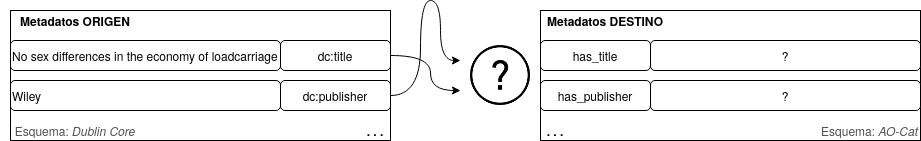
\includegraphics{../_static/images/mappingProblem.png}
\caption{Conflicto entre esquemas de metadatos
distintos}\label{mappingProblem}
}
\end{figure}

Además, un esquema está formado por un conjunto de elementos, cada uno
de los cuales está sujeto a unas determinadas reglas. Por ejemplo,
podría especificarse el tipo de dato que almacena (\emph{string},
\emph{date}, etc.) o considerarse como imprescindible (no nulo). Este
hecho aumenta aún más la complejidad del problema de integración ya que
cada miembro cuenta con sus propios elementos y con sus propias reglas.

Para dar solución a todos estos problemas, ARIADNEplus propone dividir
el proceso de integración en 6 fases.

\begin{figure}
\hypertarget{integrationPhases}{%
\centering
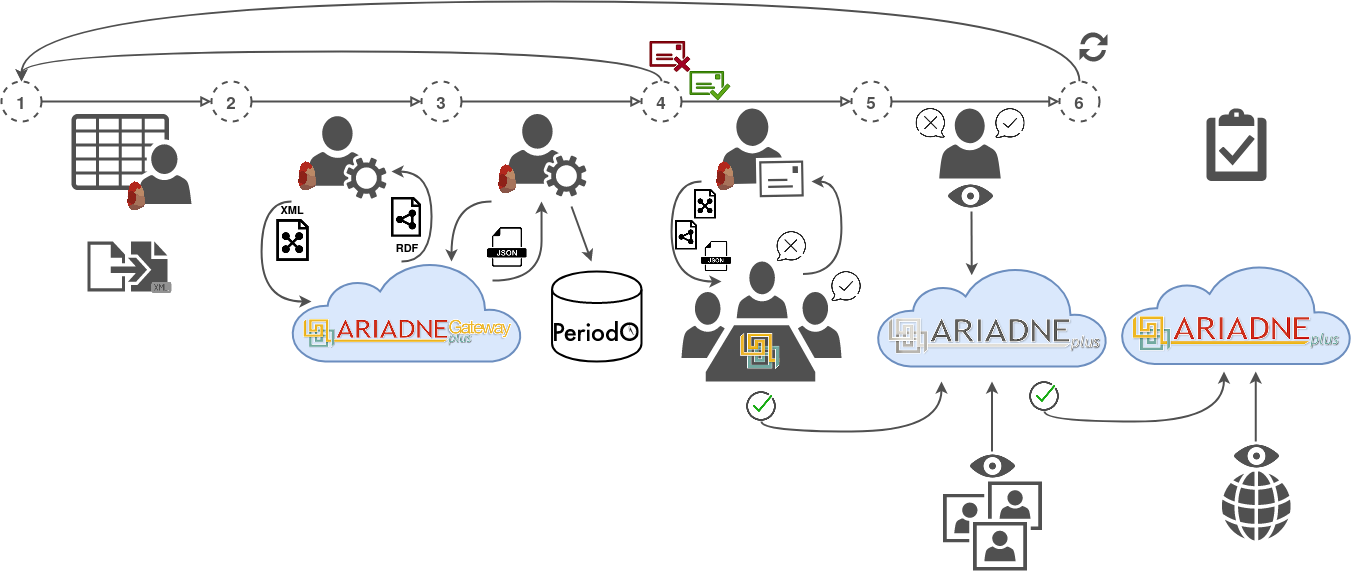
\includegraphics{../_static/images/integrationPhases.png}
\caption{Fases en las que se divide el proceso de
integración}\label{integrationPhases}
}
\end{figure}

\begin{enumerate}
\def\labelenumi{\arabic{enumi}.}
\tightlist
\item
  \textbf{Confirmación}: se confirman las colecciones de metadatos que
  serán agregadas y, además, se indica a qué categoria de datos de
  ARIADNEplus pertenecen.
\item
  \textbf{Transformación}: una vez estén listos los metadatos de origen,
  se genera un fichero de definición de mapeo que permita transformar el
  esquema de metadatos de origen al esquema objetivo (AO-Cat).
\item
  \textbf{Enriquecimiento}: se mejora la calidad de los metadatos
  sometiendo los datos a un proceso de enriquecimiento utilizando el
  vocabulario \emph{Getty AAT} y/o \emph{PeriodO}.
\item
  \textbf{Importación}: habiendo completado las tres fases anteriores,
  se ejecuta el proceso de importación de los metadatos.
\item
  \textbf{Simulación de publicación}: con los metadatos de origen ya
  importados en la base de datos, se realiza una simulación de
  publicación.
\item
  \textbf{Publicación}: si los resultados obtenidos en la fase 5 son
  favorables, se lleva a cabo la publicación de los metadatos en el
  catálogo oficial.
\end{enumerate}

\hypertarget{confirmaciuxf3n}{%
\subsubsection{Confirmación}\label{confirmaciuxf3n}}

En esta fase se confirman qué colecciones de datos serán integradas en
el proyecto. Además, se debe indicar a qué categoría de datos de ARIADNE
pertenecen.

\begin{figure}
\hypertarget{categoriesARIADNE}{%
\centering
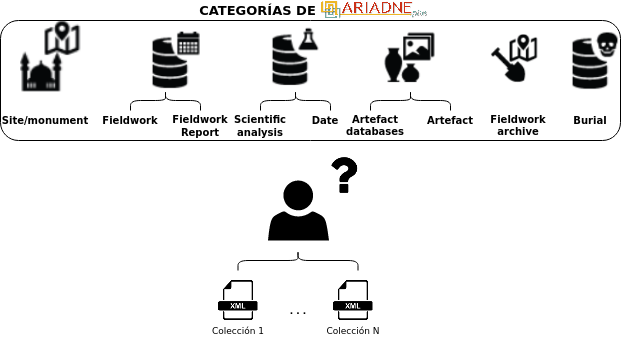
\includegraphics{../_static/images/categoriesARIADNE.png}
\caption{Fase de confirmación}\label{categoriesARIADNE}
}
\end{figure}

Afortunadamente, los datos propuestos se obtuvieron con suma facilidad,
sin ningún tipo de reticencia por parte del CENIEH. En la siguiente
tabla se indican las principales características de cada una de las
colecciones de datos confirmadas para la integración con ARIADNEplus.
Además, se especifica la categoría ARIADNE a la que corresponden.

\begin{longtable}[]{@{}llllll@{}}
\caption{Colecciones de metadatos propuestas por el CENIEH para la
integración con ARIADNEplus.}\tabularnewline
\toprule
Colección & Núm. Registros & Docs asociados & Campos & Formato &
Categoría ARIADNE\tabularnewline
\midrule
\endfirsthead
\toprule
Colección & Núm. Registros & Docs asociados & Campos & Formato &
Categoría ARIADNE\tabularnewline
\midrule
\endhead
\begin{minipage}[t]{0.14\columnwidth}\raggedright
Anatomía Comparada\strut
\end{minipage} & \begin{minipage}[t]{0.14\columnwidth}\raggedright
\begin{quote}
571
\end{quote}\strut
\end{minipage} & \begin{minipage}[t]{0.14\columnwidth}\raggedright
\begin{quote}
Sí
\end{quote}\strut
\end{minipage} & \begin{minipage}[t]{0.14\columnwidth}\raggedright
SIGNA\_CENIEH, Clase, Orden, Familia Género, Especie, Sigla de campo,
Elemento, Sexo, Adulto Localidad, Municipio, Provincia, Pais, Tipo de
objeto\strut
\end{minipage} & \begin{minipage}[t]{0.14\columnwidth}\raggedright
\begin{quote}
CSV
\end{quote}\strut
\end{minipage} & \begin{minipage}[t]{0.14\columnwidth}\raggedright
Scientific analysis\strut
\end{minipage}\tabularnewline
\begin{minipage}[t]{0.14\columnwidth}\raggedright
\begin{quote}
Litoteca
\end{quote}\strut
\end{minipage} & \begin{minipage}[t]{0.14\columnwidth}\raggedright
\begin{quote}
99
\end{quote}\strut
\end{minipage} & \begin{minipage}[t]{0.14\columnwidth}\raggedright
\begin{quote}
Sí
\end{quote}\strut
\end{minipage} & \begin{minipage}[t]{0.14\columnwidth}\raggedright
Afloramiento, Sigla, Localización, Datum, X, Y, Z, Acceso, Tipo de
Afloramiento, Tipo de roca, Depositante, Muestra física, Lámina delgada,
Laboratorio geología CENIEH, Fotografías, Otros datos, Topografía\strut
\end{minipage} & \begin{minipage}[t]{0.14\columnwidth}\raggedright
\begin{quote}
CSV
\end{quote}\strut
\end{minipage} & \begin{minipage}[t]{0.14\columnwidth}\raggedright
Scientific analysis\strut
\end{minipage}\tabularnewline
\begin{minipage}[t]{0.14\columnwidth}\raggedright
\begin{quote}
Ratón Pérez
\end{quote}\strut
\end{minipage} & \begin{minipage}[t]{0.14\columnwidth}\raggedright
\begin{quote}
1323
\end{quote}\strut
\end{minipage} & \begin{minipage}[t]{0.14\columnwidth}\raggedright
\begin{quote}
Sí
\end{quote}\strut
\end{minipage} & \begin{minipage}[t]{0.14\columnwidth}\raggedright
Sigla, Individuo, Sexo, Edad, Pieza, Superior/inferior, Lado,
Conservación, Consolidado, Pegado, Observaciones, Localización, Fecha
MicroCT, Archivo mCT, Proyecto Amira, localización, No Imágenes, kv/mA,
Vxl, Size, Filter, Fotos mCT\strut
\end{minipage} & \begin{minipage}[t]{0.14\columnwidth}\raggedright
\begin{quote}
CSV
\end{quote}\strut
\end{minipage} & \begin{minipage}[t]{0.14\columnwidth}\raggedright
Scientific analysis\strut
\end{minipage}\tabularnewline
\begin{minipage}[t]{0.14\columnwidth}\raggedright
\begin{quote}
Sedimentos
\end{quote}\strut
\end{minipage} & \begin{minipage}[t]{0.14\columnwidth}\raggedright
\begin{quote}
7695
\end{quote}\strut
\end{minipage} & \begin{minipage}[t]{0.14\columnwidth}\raggedright
\begin{quote}
No
\end{quote}\strut
\end{minipage} & \begin{minipage}[t]{0.14\columnwidth}\raggedright
ReferenciaBolsa, ReferenciaCaja, Yacimiento, Nivel, Cuadro, Z,
Situacion, FechaRecogida, FechaAlmacen, FechaProcesando\strut
\end{minipage} & \begin{minipage}[t]{0.14\columnwidth}\raggedright
\begin{quote}
CSV
\end{quote}\strut
\end{minipage} & \begin{minipage}[t]{0.14\columnwidth}\raggedright
Scientific analysis\strut
\end{minipage}\tabularnewline
\begin{minipage}[t]{0.14\columnwidth}\raggedright
\begin{quote}
CIR
\end{quote}\strut
\end{minipage} & \begin{minipage}[t]{0.14\columnwidth}\raggedright
\begin{quote}
1853
\end{quote}\strut
\end{minipage} & \begin{minipage}[t]{0.14\columnwidth}\raggedright
\begin{quote}
Sí
\end{quote}\strut
\end{minipage} & \begin{minipage}[t]{0.14\columnwidth}\raggedright
\emph{Dublin Core terms}\strut
\end{minipage} & \begin{minipage}[t]{0.14\columnwidth}\raggedright
\begin{quote}
CSV
\end{quote}\strut
\end{minipage} & \begin{minipage}[t]{0.14\columnwidth}\raggedright
Scientific analysis\strut
\end{minipage}\tabularnewline
\bottomrule
\end{longtable}

\hypertarget{transformaciuxf3n}{%
\subsubsection{Transformación}\label{transformaciuxf3n}}

Para evitar el problema mostrado en la \texttt{mappingProblem},
ARIADNEplus pone a disposición de sus miembros la \textbf{herramienta
X3ML Mapping Tool}, disponible en el VRE \emph{ARIADNEplus Mappings} del
portal \emph{ARIADNEplus Gateway} de \emph{D4Science}. Está compuesta
por un conjunto de microservicios, de código abierto, que siguen el
modelo de referencia \emph{SYNERGY} para la transmisión y agregación de
datos.

\begin{figure}
\hypertarget{transformARIADNE}{%
\centering
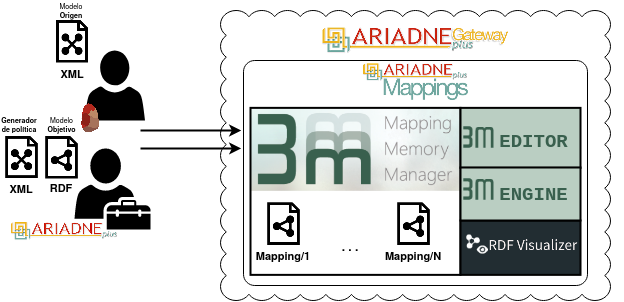
\includegraphics{../_static/images/transformARIADNE.png}
\caption{Fase de transformación}\label{transformARIADNE}
}
\end{figure}

Los componentes clave de este servicio son:

\begin{itemize}
\tightlist
\item
  \emph{3M -- Mapping Memory Manager}: herramienta utilizada para la
  gestión de archivos de definición de mapeo. Proporciona una serie de
  acciones administrativas que ayudan a los proveedores de datos a
  administrar sus archivos de definición de mapeo.
\end{itemize}

\begin{figure}
\hypertarget{mmm3m}{%
\centering
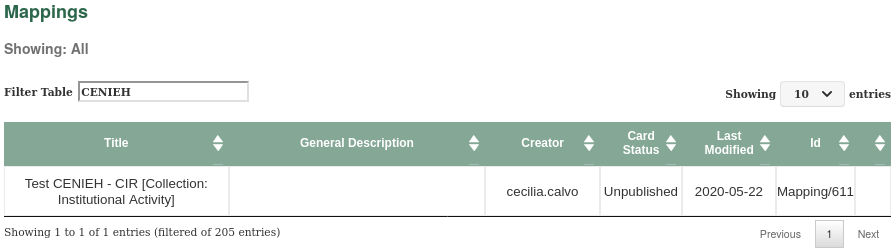
\includegraphics{../_static/images/mmm3m.png}
\caption{Vista de la herramienta \emph{Mapping Memory Manager -
3M}}\label{mmm3m}
}
\end{figure}

\begin{itemize}
\tightlist
\item
  \emph{3M Editor}: provee la interfaz que permite crear asignaciones
  entre los elementos del esquema de metadatos a mapear y el esquema
  objetivo.
\end{itemize}

\begin{figure}
\hypertarget{3meditor}{%
\centering
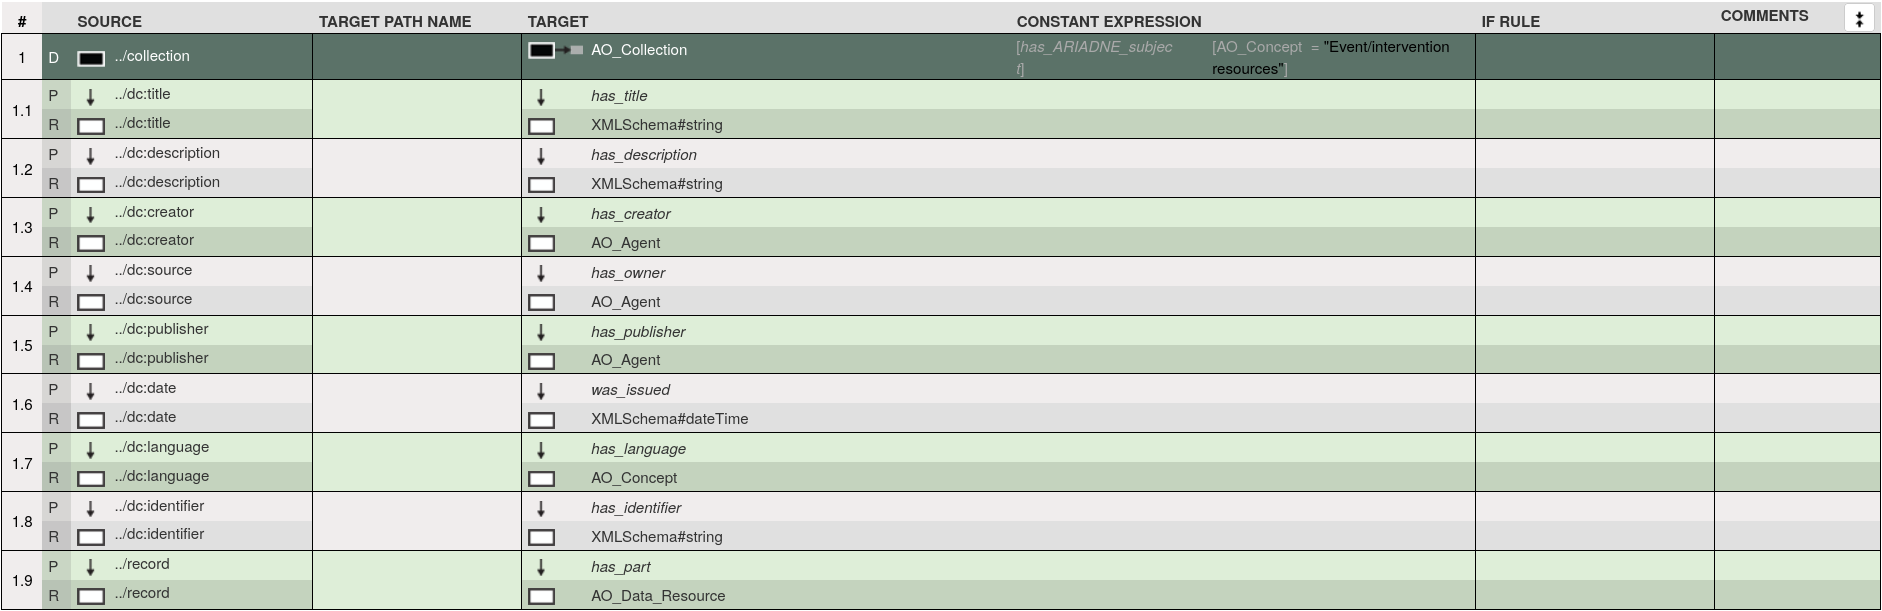
\includegraphics{../_static/images/3meditor.png}
\caption{Vista de la herramienta \emph{3M Editor}}\label{3meditor}
}
\end{figure}

\begin{itemize}
\tightlist
\item
  \emph{X3ML Engine}: ejecuta la transformación de los elementos de
  origen al formato de destino. Tomando como entrada los datos de origen
  (en formato XML), la descripción de las asignaciones existentes en el
  fichero de definición de mapeo y el archivo que contiene las políticas
  para la generación de URIs, es responsable de transformar el documento
  original en un documento RDF válido que corresponda al archivo XML de
  entrada con las asignaciones y políticas indicadas.
\item
  \emph{RDF visualizer}: permite, de una forma rápida, inspeccionar los
  documentos transformados.
\end{itemize}

\begin{figure}
\hypertarget{rdfvisualizer}{%
\centering
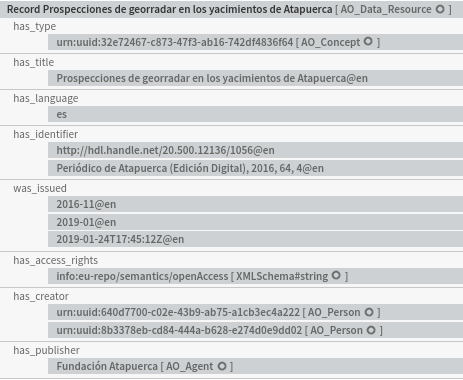
\includegraphics{../_static/images/rdfvisualizer.png}
\caption{Vista de la herramienta \emph{RDF
visualizer}}\label{rdfvisualizer}
}
\end{figure}

Esta herramienta toma un \textbf{papel decisivo} en el proceso de
integración ya que permite transformar el modelo de origen al esquema de
metadatos utilizado en ARIADNEplus (AO-CAT).

A continuación se van a describir los principales \textbf{retos} a los
que nos hemos tenido que enfrentar durante esta segunda fase:

\begin{itemize}
\tightlist
\item
  Todos los conjuntos de datos propuestos por el CENIEH están en formato
  CSV. Esto supone un problema ya que \textbf{ARIADNEplus solo trabaja
  con ficheros XML}, es decir, no cuenta con ningún método de
  importación que tolere archivos CSV.
\item
  \textbf{Los conjuntos de datos del CENIEH}, a excepción de la
  colección del CIR, están dispuestos de forma irregular, es decir,
  \textbf{no siguen ningún esquema estandarizado}. Esto implica que para
  cada conjunto de datos, se necesita hacer un fichero de definición de
  mapeo distinto, lo que no es para nada eficiente.
\item
  En el esquema objetivo, los \textbf{elementos} pueden ser opcionales u
  \textbf{obligatorios}. Los elementos opcionales no suponen ningún
  problema ya que pueden quedar vacíos, sin embargo, los elementos
  obligatorios requieren la existencia de un elemento en el modelo de
  origen que pueda sustituirlo, es decir, que tenga el mismo
  significado. Esta regla supone un reto para el CENIEH ya que muchos de
  los elementos obligatorios no cuentan con un elemento apto en las
  colecciones de datos propuestas.
\item
  \textbf{El contenido} almacenado en cada elemento del esquema objetivo
  \textbf{ha de tener un formato específico}. Por ejemplo, el contenido
  del elemento \emph{has\_language}, responsable de indicar el idioma en
  el que está dispuesto el objeto al que referencia, debe cumplir con el
  estándar ISO639-1 o ISO639-2. Por tanto, el elemento asignado en el
  origen debe seguir el mismo formato.
\end{itemize}

\hypertarget{enriquecimiento}{%
\subsubsection{Enriquecimiento}\label{enriquecimiento}}

En ocasiones, los metadatos por si solos no son lo suficientemente
precisos o claros como para describir una determinada característica del
objeto al que se refieren. En el caso de la arqueología, existen
multitud de conceptos con un alto grado de complejidad que necesitan ser
explicados en detalle. Por este motivo, ARIADNEplus propone enriquecer
los metadatos haciendo uso del vocabulario \emph{Getty AAT} y del
cliente \emph{PeriodO}.

\begin{figure}
\hypertarget{enrichment}{%
\centering
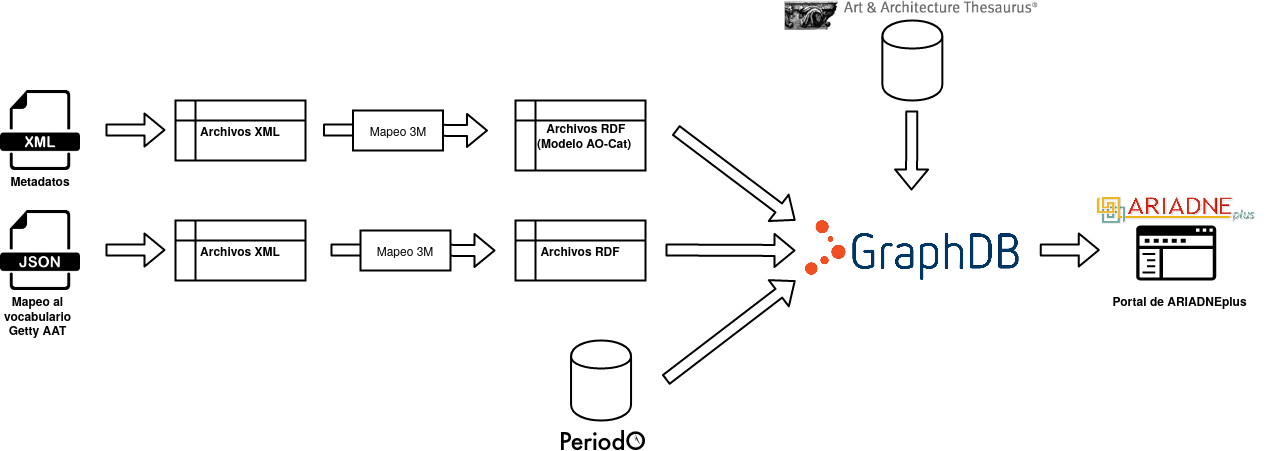
\includegraphics{../_static/images/enrichment.png}
\caption{Enriquecimiento de metadatos}\label{enrichment}
}
\end{figure}

En la \texttt{enrichment} se muestra el flujo de datos del proceso de
enriquecimiento de metadatos. Por una parte, vemos un archivo .json, el
cual se obtiene a través de la \textbf{herramienta Vocabulary Matching
Tool}. Esta es otra de las herramientas que se pueden encontrar en el
VRE \emph{ARIADNEplus Mappings}. Permite mapear el vocabulario utilizado
en el documento de origen al vocabulario \emph{Getty AAT}.

\begin{figure}
\hypertarget{vmt}{%
\centering
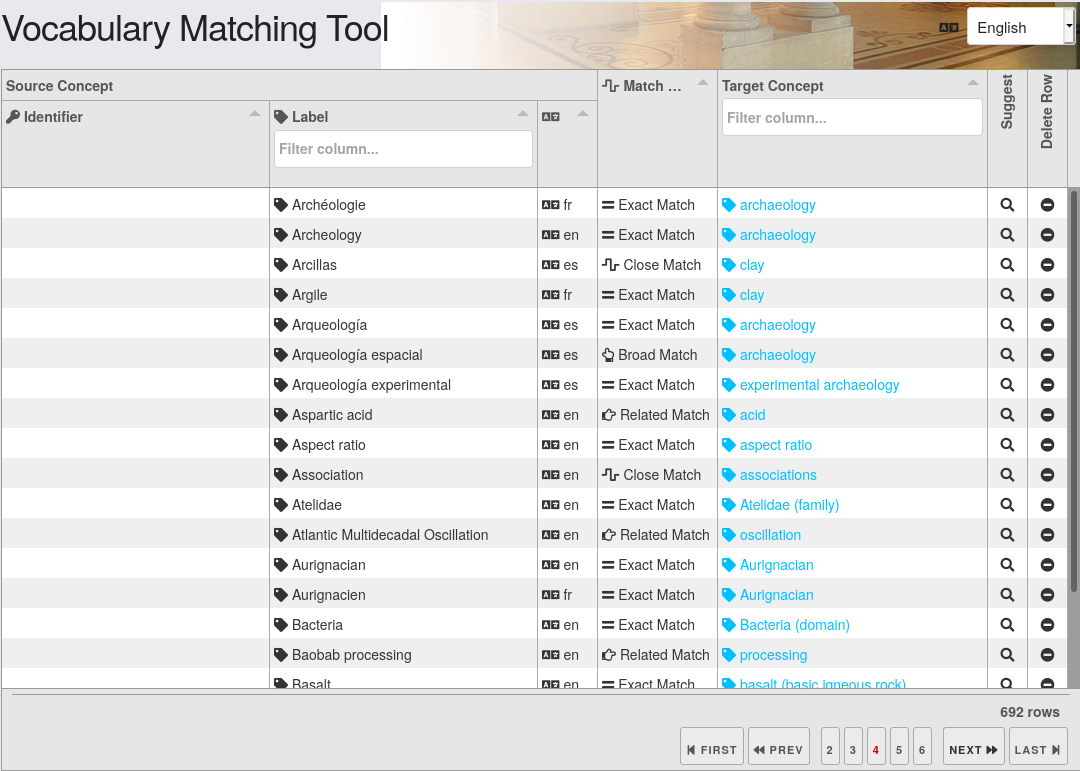
\includegraphics{../_static/images/vmt.png}
\caption{Vista de la herramienta \emph{Vocabulary Matching
Tool}}\label{vmt}
}
\end{figure}

El archivo generado por esta herramienta (.json) define las relaciones
entre los conceptos del vocabulario de origen y los conceptos del
vocabulario \emph{Getty AAT}. Desde el catálogo de ARIADNEplus, todos
aquellos términos que tengan una asociación definida, serán hiperenlaces
que apunten al concepto Getty AAT asociado.

Además, vemos representada la BD donde \textbf{PeriodO} almacena sus
registros. Para aportar información adicional a los periodos existentes
en nuestros datos, debemos publicar en el cliente de PeriodO nuestra
propia colección de periodos. De esta forma, ARIADNEplus podrá recoger
desde la BD de periodO nuestra colección para, posteriormente,
establecer una relación entre los periodos de un lado y de otro. Al
igual que con el vocabulario, todos los periodos que tengan una
asociación definida, serán hiperenlaces que apunten al objeto de
periodO.

En esta fase se encontraron varios \textbf{inconvenientes}: - Muchos de
los términos existentes en los conjuntos de datos del CENIEH no están
presentes en el vocabulario \emph{Getty AAT}. Por este motivo, solo se
pudo enriquecer una pequeña parte del conjunto total. - Para poder
publicar la colección en periodO, se requería determinar la autoridad de
los periodos, es decir, indicar de donde procedían. Desde el CENIEH no
me pudieron facilitar ese dato ya que lo desconocían. Por este motivo,
no se pudo llevar a cabo la publicación y por ende no se enriquecerieron
los periodos.

\hypertarget{importaciuxf3n}{%
\subsubsection{Importación}\label{importaciuxf3n}}

El sistema de importación de ARIADNEplus, conocido como ARIADNEplus
\emph{Aggregator}, se basa en el kit de herramientas de \emph{software}
D-Net (implementado y mantenido por ISTI-CNR\footnote{"ISTI-CNR --
  Istituto di Scienza e Tecnologie dell'Informazione "
  \url{https://www.isti.cnr.it/}}), que proporciona funciones integradas
que permiten recopilar conjuntos de metadatos a través de múltiples
métodos. Está disponible en el portal \emph{ARIADNEplus Gateway}, sin
embargo, su acceso está restringido a los coordinadores del proyecto.
Las principales opciones son:

\begin{enumerate}
\def\labelenumi{\arabic{enumi}.}
\tightlist
\item
  \textbf{OAI-PMH}: es un protocolo estándar para el intercambio de
  metadatos. A través de este método ARIADNEplus puede recopilar todo el
  contenido o los conjuntos de datos OAI que le indiquemos.
\item
  \textbf{SFTP}: es un protocolo de transmisión de ficheros. Esta opción
  es algo engorrosa ya que debe existir un archivo XML por recurso, es
  decir, no puedes agrupar varios registros en un mismo fichero XML. Los
  socios son responsables del servidor SFTP. Se admiten modos de
  autentificación.
\item
  \textbf{FTP(S)}: es otro protocolo de transferencia de ficheros.
  Presenta las mismas características de importación que SFTP.
\item
  \textbf{Workspace}: se pueden subir directamente los registros en el
  \emph{workspace} de D4Sciente (ARIADNEplus Gateway). Cada socio tiene
  su propia carpeta donde puede ir almacenando los documentos XML
  (metadatos) que desee importar.
\end{enumerate}

Dado que este sistema es inaccesible para la mayoría de los miembros
(incluido el CENIEH), se debe escoger una de esas opciones y
comunicársela al coordinador responsable. Una vez realizada la
importación, se deben facilitar tres datos:

\begin{itemize}
\tightlist
\item
  Qué ficheros (\emph{.xml}) de los importados se desean publicar.
\item
  Cuál es el identificador del fichero de definición de mapeo (e.g.
  \emph{Mapping/621}) que transformará el esquema de metadatos presente
  en tus ficheros al esquema AO-Cat.
\item
  Opcionalmente, el enlace a tu colección de periodO y/o el fichero de
  mapeo (\emph{.json}) del vocabulario.
\end{itemize}

Los conjuntos de datos del CENIEH están almacenados de forma local,
exceptuando el CIR. Por ello, de entre todas las opciones posibles, la
única forma válida de importar metadatos sería a través del
\emph{Workspace}.

\hypertarget{simulaciuxf3n-de-publicaciuxf3n}{%
\subsubsection{Simulación de
publicación}\label{simulaciuxf3n-de-publicaciuxf3n}}

Una vez establecida la comunicación con el coordinador responsable del
proceso de importación, se debe esperar a su respuesta. Dependiendo del
contenido de la respuesta, se pueden tomar dos caminos:

\begin{enumerate}
\def\labelenumi{\arabic{enumi}.}
\tightlist
\item
  Nos indican que todas las partes del proceso (metadatos, mapeo,
  enriquecimiento) son correctos. En tal caso, los metadatos propuestos
  estarían ya disponibles desde el portal fantasma de ARIADNEplus. Este
  es idéntico al original con la única diferencia de que sólo tienen
  acceso los miembros del proyecto.
\item
  Nos indican que alguna parte del proceso no es correcta. Ante esta
  situación, se debe volver hacia atrás en el proceso de integración
  para solventar los conflictos señalados por el coordinador.
\end{enumerate}

\hypertarget{publicaciuxf3n}{%
\subsubsection{Publicación}\label{publicaciuxf3n}}

Si en la fase previa se ha obtenido una respuesta satisfactoria, el
miembro que inició el proceso de integración sería ya capaz de observar
el resultado final. A continuación, deberá comunicarse de nuevo con el
responsable de la importación para indicarle sus impresiones. Se pueden
dar dos situaciones:

\begin{enumerate}
\def\labelenumi{\arabic{enumi}.}
\tightlist
\item
  El resultado es favorable. Ante esta situación el coordinador lleva a
  cabo la publicación de los datos en el portal original.
\item
  No se esperaba el resultado obtenido. En tal caso, se deben mantener
  las conversaciones hasta llegar a una solución.
\end{enumerate}

En el caso de que todo haya salido según lo planeado, el proceso de
integración para los conjuntos de datos publicados quedaría suspendido.
Existe la posibilidad de reactivar este proceso en el caso de que se
deseen actualizar ciertos datos, sin embargo, hay que tener en cuenta
que cualquier cambio en la estructura de los datos supondría tener que
volver a realizar el proceso desde 0.

\hypertarget{desarrollo}{%
\section{Desarrollo}\label{desarrollo}}

Recordemos que en la fase anterior se anotaron todos los aspectos
relevantes del proceso de integración, incluyendo además los problemas
de incompatibilidad encontrados entre dicho proceso y los datos
propuestos por el CENIEH. Es en esta fase cuando se aplican las
competencias y los conocimientos adquiridos a lo largo del grado con el
objetivo de desarrollar una infraestructura \emph{software} que sea
capaz de guiar a los operarios del CENIEH en el proceso de integración
y, además, resuelva los problemas mencionados en la fase anterior.

\hypertarget{omeka-como-aplicaciuxf3n-principal}{%
\subsection{\texorpdfstring{\emph{Omeka} como aplicación
principal}{Omeka como aplicación principal}}\label{omeka-como-aplicaciuxf3n-principal}}

Desarrollar desde cero una infraestructura \emph{software} que cumpliera
con todos los requisitos propuestos no era viable debido a la limitación
temporal del proyecto. Por este motivo, se decidió utilizar
\emph{software} de terceros que cumpliera con un mínimo de
\textbf{requisitos}:

\begin{itemize}
\tightlist
\item
  Permitir la \textbf{gestión de metadatos}: los archivos de información
  involucrados son metadatos, por tanto, se necesita un sistema que
  permita realizar todo tipo de tareas de gestión sobre este tipo de
  datos.
\item
  Disponer de \textbf{herramientas de importación y exportación}: los
  datos de origen necesitarán ser importados a la plataforma para
  realizar sobre ellos las operaciones oportunas. Una vez gestionados,
  deberán ser exportados para someterlos al proceso de integración.
\item
  Ser \textbf{software libre}: este requisito era fundamental ya que,
  para poder adaptar la infraestructura a las necesidades del proyecto,
  se debe tener total libertad a la hora de ejecutar, copiar,
  distribuir, estudiar, modificar y mejorar el \emph{software}.
\end{itemize}

Se consideraron varios productos \emph{software} para acabar escogiendo
\href{https://omeka.org/classic/}{Omeka Classic}. Una de las
características que hacen de la aplicación una magnífica plataforma para
el proyecto es su \textbf{escalabilidad}. Gracias a su sistema de
\textbf{complementos} o \emph{plugins}, cualquier programador tiene la
posibilidad de adaptarla a sus necesidades individuales sin necesidad de
modificar el código base de la aplicación.

Actualmente, \emph{Omeka} cuenta con una gran cantidad de \emph{plugins}
disponibles tanto en su \href{https://omeka.org/classic/plugins/}{página
oficial} como en
\href{https://daniel-km.github.io/UpgradeToOmekaS/omeka_plugins.html}{Github}.
Esto es posible gracias a la extensa comunidad de usuarios que le
respalda. Parte de esos \emph{plugins} se han podido utilizar para
adaptar la infraestructura a las necesidades del proyecto, sin embargo,
se han tenido que desarrollar nuevos \emph{plugins} para cubrir
requisitos específicos. Además, se han llevado a cabo modificaciones
sobre alguno de los \emph{plugins} de terceros utilizados.

Por tanto, parte de las tareas de esta fase están relacionadas con la
creación y modificación de \emph{plugins} para \emph{Omeka}.

\hypertarget{adaptaciuxf3n-de-la-plataforma}{%
\subsubsection{Adaptación de la
plataforma}\label{adaptaciuxf3n-de-la-plataforma}}

Los complementos o \emph{plugins} son capaces de añadir nuevas
funcionalidades a \emph{Omeka} gracias a que esta tiene implementado un
sistema de ganchos o \emph{hooks}. Estos nos permiten acoplar código en
puntos específicos del flujo de ejecución de la aplicación, evitando así
tener que alterar el código base de esta.

Dentro de la aplicación se pueden encontrar dos tipos distintos de
\emph{hooks}: \emph{hooks} de acción y filtros (\emph{filters}).

\hypertarget{hooks-de-acciuxf3n}{%
\paragraph{\texorpdfstring{\emph{Hooks} de
acción}{Hooks de acción}}\label{hooks-de-acciuxf3n}}

Este tipo de \emph{hook} permite añadir la ejecución de funciones en
puntos de ejecución específicos.

Por ejemplo, en el caso de que se quiera introducir un formulario en una
página de \emph{Omeka}, se debería utilizar el \emph{action hook}
alojado en dicha página para ejecutar la función encargada de imprimir
el código HTML del formulario. En este ejemplo, la función no retornaría
nada ya que se limita a imprimir código, y es que en este tipo de
\emph{hooks} la función no tiene por qué devolver nada.

En los archivos de Omeka se pueden localizar estos \emph{hooks} buscando
la función \emph{fire\_plugin\_hook()}. Una vez encontrada, desde el
\emph{plugin} que estamos desarrollando, haciendo uso de la interfaz
\emph{Omeka\_Plugin\_AbstractPlugin}, bastaría con añadir este
\emph{hook} a la lista \emph{\_hooks} e instanciar el método
correspondiente, el cual siempre tiene la nomenclatura
\emph{hook\textless NombreDelHook\textgreater()}.

\begin{figure}
\hypertarget{actionhooks}{%
\centering
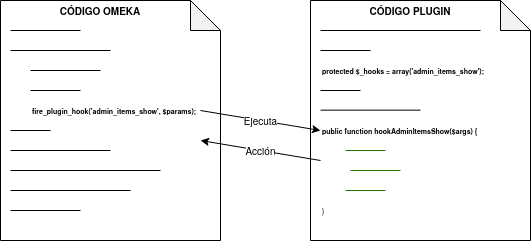
\includegraphics{../_static/images/actionhooks.png}
\caption{Ejemplo de hook de acción}\label{actionhooks}
}
\end{figure}

En el ejemplo vemos como \emph{fire\_plugin\_hook()} tiene dos
parámetros de entrada, el primero indica el nombre del \emph{hook} y el
segundo almacena los argumentos de entrada que tendrá la función que
almacena la acción.

\hypertarget{filtros-filters}{%
\paragraph{\texorpdfstring{Filtros
(\emph{Filters})}{Filtros (Filters)}}\label{filtros-filters}}

Los filtros permiten, al igual que los \emph{hooks} de acción, ejecutar
funciones propias en puntos específicos de la aplicación. Sin embargo,
el objetivo de estos es algo distinto ya que no pretenden modificar
código sino alterar los datos de una determinada variable.

Las funciones implicadas deben tener un parámetro de entrada y otro de
salida de forma que, desde el interior de la función, se procesa el
valor de entrada y se devuelve el valor resultante.

En los archivos de \emph{Omeka} se pueden localizar estos \emph{hooks}
buscando la función \emph{apply\_filters()}. Una vez encontrada, existen
dos formas de usar ese filtro:

\begin{enumerate}
\def\labelenumi{\arabic{enumi}.}
\tightlist
\item
  Utilizando la interfaz \emph{Omeka\_Plugin\_AbstractPlugin} es posible
  utilizar el filtro añadiendo su nombre a la lista \emph{\_filters}. A
  continuación, se añadiría el método público con el nombre
  \emph{filter} seguido del nombre del filtro.
\end{enumerate}

\begin{figure}
\hypertarget{filterhooksA}{%
\centering
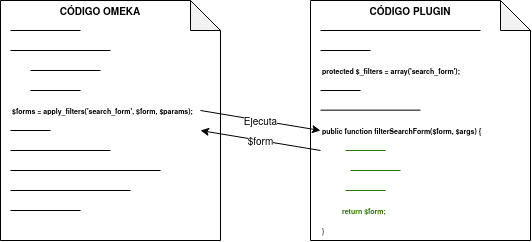
\includegraphics{../_static/images/filterhooksA.png}
\caption{Ejemplo de \emph{filter hook}}\label{filterhooksA}
}
\end{figure}

\begin{enumerate}
\def\labelenumi{\arabic{enumi}.}
\setcounter{enumi}{1}
\tightlist
\item
  Utilizando el método \emph{add\_filter()}, se puede utilizar el filtro
  pasando como primer parámetro el nombre del filtro implicado y como
  segundo parámetro la función que se ejecutará. En este caso, el nombre
  de la función es personalizable. Además, se puede pasar un tercer
  parámetro para indicar la prioridad de nuestro \emph{hook}, es decir,
  si existiera más de un \emph{plugin} utilizando ese mismo filtro, se
  ejecutaría la función de cada uno en función de su prioridad, de mayor
  a menor prioridad. Por defecto, todos los \emph{filtros} de cada
  \emph{plugin} tienen una prioridad de 10, por lo que el orden de
  ejecución se determina por la fecha de instalación, de más antiguos a
  más nuevos.
\end{enumerate}

\begin{figure}
\hypertarget{filterhooksB}{%
\centering
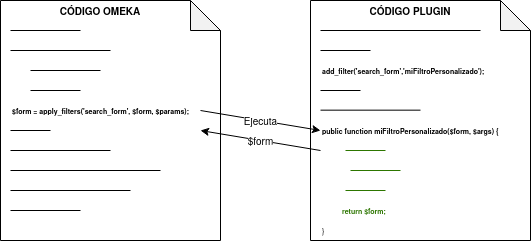
\includegraphics{../_static/images/filterhooksB.png}
\caption{Segundo ejemplo de \emph{filter hook}}\label{filterhooksB}
}
\end{figure}

\hypertarget{entornos-de-trabajo}{%
\subsection{Entornos de trabajo}\label{entornos-de-trabajo}}

Durante la fase de desarrollo, se ha trabajado sobre dos entornos:

\begin{itemize}
\tightlist
\item
  \textbf{Entorno de desarrollo}: se actualiza al cometer cambios sobre
  la rama \emph{develop}. Permite llevar un seguimiento diario del
  estado de la aplicación durante el desarrollo de la misma. Es público.
\item
  \textbf{Entorno de producción}: se actualiza al cometer cambios sobre
  la rama \emph{main}. En su interior se puede encontrar una versión
  estable de la aplicación. El intervalo de tiempo de actualización gira
  entorno a las dos semanas. Es privado, sólo tienen acceso los miembros
  del CENIEH.
\end{itemize}

\hypertarget{despliegue-de-la-infraestructura}{%
\subsection{Despliegue de la
infraestructura}\label{despliegue-de-la-infraestructura}}

Para llevar a cabo el despliegue de la infraestructura se ha utilizado
la herramienta \emph{Github Actions}. Dependiendo del entorno de
trabajo, se ha procedido de una manera u otra:

\hypertarget{servidor-de-desarrollo}{%
\subsubsection{Servidor de desarrollo}\label{servidor-de-desarrollo}}

A través de la herramienta \emph{Github Actions} se ha automatizado el
despliegue de la infraestructura sobre el servidor de desarrollo. A esta
técnica se la conoce como despliegue continuo.

\begin{figure}
\hypertarget{cicd}{%
\centering
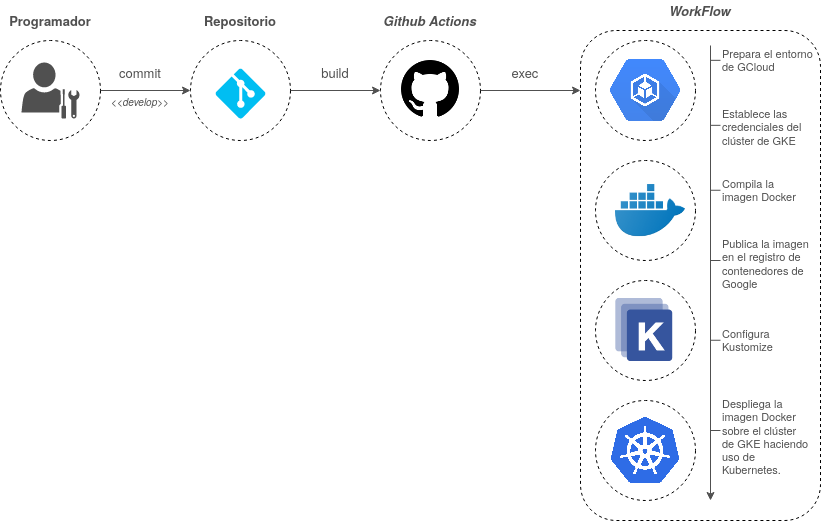
\includegraphics{../_static/images/cicd.png}
\caption{Despliegue continuo de la aplicación}\label{cicd}
}
\end{figure}

En la \texttt{cicd} he representado el proceso mediante el cual se lleva
a cabo el despliegue. Con el \emph{workflow} configurado y alojado en la
ruta \emph{.github/workflows} de mi repositorio en GitHub, cuando
ejecuto un \emph{push} sobre la rama \emph{develop}, si los cambios
cometidos afectan a cualquier carpeta que no sea la de \emph{/docs}, se
ejecutan las acciones correspondientes al despliegue de mi aplicación,
las cuales se pueden apreciar en la imagen.

\hypertarget{servidor-de-producciuxf3n}{%
\subsubsection{Servidor de producción}\label{servidor-de-producciuxf3n}}

Sobre el servidor de producción no se ha podido automatizar el
despliegue debido a que el acceso a este era privado, es decir, no se
podía establecer comunicación desde el exterior sin previa conexión al
VPN del CENIEH y el posterior acceso vía \emph{ssh} al servidor.

\begin{figure}
\hypertarget{dockerdeploy}{%
\centering
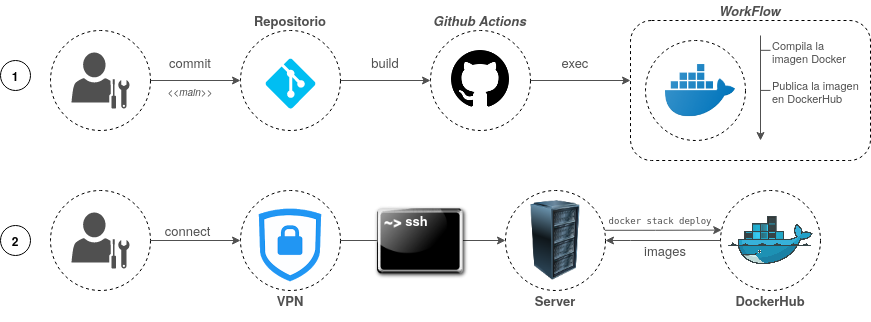
\includegraphics{../_static/images/dockerdeploy.png}
\caption{Despliegue "semi-continuo" de la
aplicación}\label{dockerdeploy}
}
\end{figure}

Como solución a este inconveniente, se automatizó por separado la
compilación y publicación de la imagen \emph{Docker} asociada a nuestra
aplicación. De esta manera, cada vez que se cometía un cambio sobre la
rama \emph{main}, se ejecutaba dicho proceso, actualizando la imagen
publicada en el repositorio de \emph{DockerHub}. Finalizado el proceso,
se accedía al servidor de producción y se desplegaba manualmente la
infraestructura. Durante el despliegue, se recogían las imágenes desde
\emph{DockerHub}, incluyendo la imagen actualizada de nuestra
aplicación.

\end{document}
